\chapter{Architecture and implementation} \label{chapter5}

Having clarified the user-facing functionalities and the general design framework for our module, we will explain the system-related features and architecture that support our news aggregator module.

\section{Flutter and ACS UPB Mobile}

\textbf{ACS UPB Mobile} is implemented using the Flutter framework from Google, and the app's most recent release is stable for the \textbf{Flutter 1} version. Flutter uses the Dart object-oriented programming language and enables developers to compile their app natively to Android, iOS and the web with one single code base. The ability of targeting cross-platform systems means a larger user audience and solves the need of having separate native developer teams for each platform. \textbf{Ioana Alexandru}, the original creator of \textbf{ACS UPB Mobile}, has considered Flutter as the choice for this project upon careful and considerable comparison between this framework and other popular solutions \cite{ioana-alexandru-flutter-choice}, such as \textit{Xamarin}\footnote{https://dotnet.microsoft.com/en-us/apps/xamarin} or \textit{React Native}\footnote{https://reactnative.dev/}. Its code reusability and growing community were strong arguments among others for choosing Flutter.

~
Our news aggregator module is written using Dart. Dart supports common modern features in the current programming languages spectrum, such as type and null-safety, concurrency, platform independence, flexible compilation, browser support; and in addition, it is open-source and is backed by a large developer community.

~
Flutter developers can publish package repositories on \textit{pub.dev}\footnote{https://pub.dev/} from where these can be downloaded and used in other projects. Our app uses several such packages to achieve different functionalities, like for example, image picking\footnote{https://pub.dev/packages/image\_picker}, URL launching\footnote{https://pub.dev/packages/url\_launcher} or deep-linking\footnote{https://pub.dev/packages/uni\_links}.

\subsection{Upgrade to Flutter version 2}

Our current target SDK for Android is \textbf{version 29} on the release branch, and for several months, there have been increasing efforts to upgrade the code base of our app to \textbf{Flutter 2}. The target SDK referes to a property that "tells the system for which Android version the app was designed and tested on" \cite{targetsdk-meaning}. This upgrade is a necessary change since, according to this official Google Help post\footnote{https://support.google.com/googleplay/android-developer/answer/11926878}, new app updates must target SDK \textbf{version 30} starting with \textbf{November 1, 2021} and existing apps must meet this requirement by \textbf{November 1, 2022}. Otherwise, apps that fail this condition will no longer be available on Google Play Store for new users. 

~
Flutter 2 enables target SDK for \textbf{version 30} and forces code migration to null-safety standards. For our app to be eligible for migration, all packages used in our app must be null-safety compatible. Consequently, this involves either using packages at their latest null-safety compatible versions or replacing them with other packages altogether. Currently, there are a number of pull requests\footnote{https://github.com/student-hub/acs-upb-mobile/pulls} that await approval or reviewing, without which our migration process could not be finalized. When merged into the main branch, our news aggregator module should already be eligible for Flutter version 2.

\subsection{Code overview}

Flutter follows the declarative programming paradigm, which according to the official documentation\footnote{https://docs.flutter.dev/development/data-and-backend/state-mgmt/declarative}, "builds its user interface to reflect the current state" of the app. The following \textbf{diagram \ref{4:fig:declarative-equation}} from the official documentation\footnote{https://docs.flutter.dev/assets/images/docs/development/data-and-backend/state-mgmt/ui-equals-function-of-state.png} illustrates this concept. This programming paradigm is different from the imperative framework because it focuses on the desired output rather than on the processes and actions that lead to that output. The crucial element of the declarative framework is the state, and each state change triggers the rebuilding of the UI.

\begin{figure}[ht]
    \centering
    
\includegraphics[width=0.5\textwidth]{figures/app/miscellanous/ui-equals-function-of-state.png}
    \caption{Declarative paradigm equation}
    \label{4:fig:declarative-equation}
\end{figure}

~
Our Flutter UI consists of components called widgets. Everything in Flutter is a widget, and all these components are placed within a data structure called the render tree. Flutter uses \textit{aggressive composability}\footnote{https://docs.flutter.dev/resources/inside-flutter\#aggressive-composability} to compose widgets progressively out of more basic widgets. Each widget component can be stateless (it does not have a state) or stateful (it can change its internal state). When building the UI, the render tree determines which components are affected by the state changes and updates the UI accordingly. For this, Flutter uses a series of optimization techniques\footnote{https://docs.flutter.dev/resources/inside-flutter} to achieve sublinear building times and fast performances.

~
When writing our code for the news aggregator module, we followed the current code guidelines in the project.  \textbf{ACS UPB Mobile} uses a variation of the \textbf{BLoC (Business Logic Component)}\footnote{https://www.mitrais.com/news-updates/getting-started-with-flutter-bloc-pattern/} design pattern, which decouples the UI entirely from the business logic. The UI is described inside the \textbf{View} layer and regularly emits events to the \textbf{Service} layer, which is encapsulated by our business logic component. Our services contain functions that receive events and output values that can be further used in updating the View state. These services wrap the entire widget tree and, as a result, become globally accessible and reusable from any widget component. Finally, the \textbf{Data} layer responds to the asynchronous requests coming from services and uses data models for exchanging information.

\begin{figure}[ht]
    \centering
    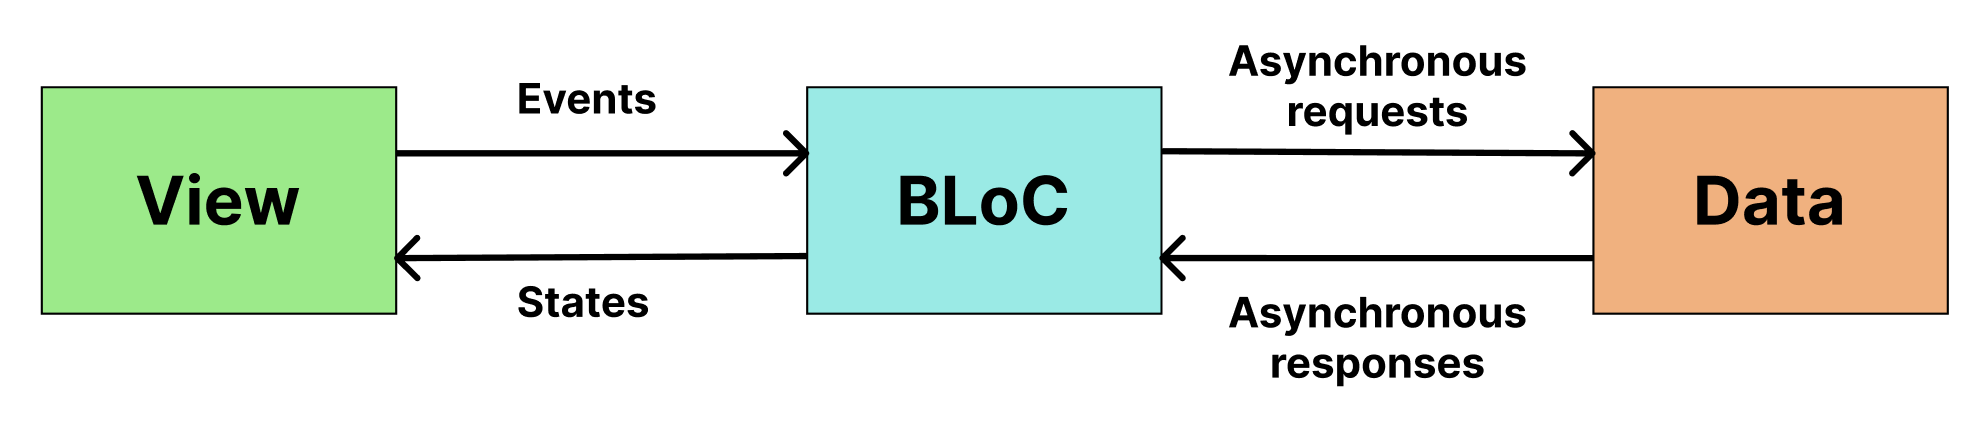
\includegraphics[width=\textwidth]{figures/app/miscellanous/bloc-diagram.png}
    \caption{BLoC diagram}
    \label{4:fig:bloc-diagram}
\end{figure}

\section{Firebase}

\textbf{ACS UPB Mobile} employs \textit{Firebase}\footnote{https://firebase.google.com/} services from Google for achieving a serverless backend infrastructure. Firebase is part of the same category as \textit{Amazon Web Services}\footnote{https://aws.amazon.com/} or \textit{Azure}\footnote{https://azure.microsoft.com/en-us/} and takes care of many common functionalities such as authentication, database, storage or cloud functions. Some of the most significant advantages of a serverless architecture are less operational complexity, a pay-as-you-go pricing model, and an autoscaling feature. Developers concern themselves less with the cloud maintenance and more with the actual functionalities they want to implement. In addition, the large documentation and available resources make for a straight-forward integration of Firebase with a wide range of projects, including with Flutter.

~
For our news aggregator module, the most relevant services we used were \textit{Firestore}\footnote{https://firebase.google.com/docs/firestore}, \textit{Firebase Cloud Functions}\footnote{https://firebase.google.com/docs/functions} and \textit{Firebase Cloud Messaging}\footnote{https://firebase.google.com/docs/cloud-messaging}. Building upon an existing project meant we did not need to concern ourselves with core functionalities, such as authentication or hosting, but instead, we could focus on directly implementing our features described in \textbf{chapter \ref{chapter4}}.

\section{Database}

During our implementation process, we worked on a different development environment to not cause any damage or unrelated changes to the production one. Moreover, data from production is regularly synced with the development database so that we can replicate issues or start testing features directly on accurate information. For our database layer, we employed Firestore, and we defined or changed several data models to accommodate our needs.

\subsection{Firestore}

According to the official documentation\footnote{https://firebase.google.com/docs/firestore}, Firestore is a NoSQL document-oriented database service with many advantages concerning performance, scaling and ease of application. Besides this, Firestore provides offline query support, local caching, security rules, and database triggers with defined cloud functions. However, it does not support aggregation queries and has certain limitations, such as 1MB document size limit or document write frequency limit of 1 per second. Nevertheless, for the purpose of \textbf{ACS UPB Mobile} and of our news aggregator module, this solution provides more than enough in terms of performance and usage. 

~
Data in Firestore is organized in collections that can hold multiple documents, and each document can have multiple sub-collections with nested sub-documents. Collections are schemaless, and documents organize their data in key-value pairs. In the following subsection \textbf{\ref{5:models}}, we will describe our collections' structure.

~
As a side note, Firestore employs security rules that govern who can read, create or modify existing data in a certain collection. The following code snippet represents an example of the syntax used. The shown example means: anyone can read all documents in the \textbf{news} collection, only authenticated users can create new documents, only the admins and the author can modify or delete a specific document. 

\begin{verbatim}
 match /news/{news} {
    allow read: if true;
    allow create: if isAuthenticated()
    allow update: if isOwner() || permissionLevel() >= 3;
    allow delete: if isOwner() || permissionLevel() >= 3;
}
\end{verbatim}

\subsection{Models} \label{5:models}

For our news aggregator module, we created new collections or modified existing ones to store all the information we needed. We had to accommodate the need to store additional user information, the data about the available news items, and the information that supports our push-notifications system described at \textbf{section \ref{5:pipeline}}.

~

\faDatabase \hspace{0.1cm} \textbf{\mintinline{text}{users}}

~
This collection stores the information related to users. Since rigorous database rules protect each user's document, we tried to fit as much information related to a user as possible in their own document and avoid using other collections. For simplicity, our model \textbf{\ref{5:tab:users}} describes only the fields that were added for the purpose of our module.

\begin{table}[th]\small\linespread{1}
    \centering
    \caption{\textbf{users} collection (only additions)}
    \label{5:tab:users}
    \begin{tabular}{| l | l | p{6.1cm} |}
    \hline
    \textbf{Field} & \textbf{Type} & \textbf{Description} \\
    \hline
    receiveNotifications & \mintinline{text}{boolean} & checks whether the user has enabled the notifications
    \\
    \hline
    roles & \mintinline{text}{array<string>} & roles that a user can select from when publishing
    \\
    \hline
    sources & \mintinline{text}{array<string>} & information source categories that the user is subscribed to
    \\
    \hline
    bookmarkedNews & \mintinline{text}{array<string>} & list of all references of news documents bookmarked by the user
    \\
    \hline
    \end{tabular}
\end{table}

~

\faDatabase \hspace{0.1cm} \textbf{\mintinline{text}{news}}

~
This collection stores all available news items and their information. Each news document contains information about the title, body, author, timestamp and other metadata that helps organize the items according to each user configuration and display them in a user-friendly manner. As a side note, the relevance field is introduced by \textbf{Ioana Alexandru} in her thesis \cite{ioana-alexandru-relevance-field} and acts as a filter by year, series, group or subgroup for students. Another use case for this relevance filter in the app is showing the proper timetable to a student based on their current year distribution. These filters can be visualized as a tree data structure, starting from less specific parent nodes that describe year or faculty to more specific leaf nodes that describe groups or subgroups.

~

\begin{table}[th]\small\linespread{1}
    \centering
    \caption{\textbf{news} collection}
    \label{5:tab:users}
    \begin{tabular}{| l | l | p{6.5cm} |}
    \hline
    \textbf{Field} & \textbf{Type} & \textbf{Description} \\
    \hline
    title & \mintinline{text}{string} & title of the post
    \\
    \hline
    body & \mintinline{text}{string} & content of a post
    \\
    \hline
    category & \mintinline{text}{string} & source information category of the post
    \\
    \hline
    categoryRole & \mintinline{text}{string} & role used by the author when publishing the post
    \\
    \hline
    relevance & \mintinline{text}{array<string>} & target student group(s) for the post (e.g. 342C3, CTI)
    \\
    \hline
    userId & \mintinline{text}{string} & reference to the author's user document
    \\
    \hline
    authorAvatarUrl & \mintinline{text}{string} & link to the author's avatar
    \\
    \hline
    authorDisplayName & \mintinline{text}{string} & author's name used when displaying the news item
    \\
    \hline
    externalLink & \mintinline{text}{string} & external reference to the original post
    \\
    \hline
    createdAt & \mintinline{text}{timestamp} & creation timestamp of the post
    \\
    \hline
    \end{tabular}
\end{table}

~

\faDatabase \hspace{0.1cm} \textbf{\mintinline{text}{fcmTokens}}

~
This collection stores tokens used in pushing notifications to devices. Each installed instance of the app on a device generates a unique registration token that helps the \textit{Firebase Cloud Messaging} service send notifications to that specific device. These tokens map devices and not authentication instances. Therefore, we need the \mintinline{text}{receiveNotifications} field from the \textbf{users} collection to check whether a user wants to receive notifications.
~

\begin{table}[th]\small\linespread{1}
    \centering
    \caption{\textbf{fcmTokens} collection}
    \label{5:tab:users}
    \begin{tabular}{| p{3.5cm} | p{2.7cm} | p{6.1cm} |}
    \hline
    \textbf{Field} & \textbf{Type} & \textbf{Description} \\
    \hline
    token & \mintinline{text}{string} & value used by Firebase when sending push-notifications
    \\
    \hline
    \end{tabular}
\end{table}

~

\faDatabase \hspace{0.1cm} \textbf{\mintinline{text}{roleRequests}}

~
This collection stores all role requests made by users and, in addition, metadata about the admin user handling these requests. For example, when a user applies for a specific role, they submit a form request mentioning the role and a reason. Afterwards, an admin accepts or declines their application, and upon acceptance, a confirmation email is sent to the user informing them of their new role. 
~

\begin{table}[th]\small\linespread{1}
    \centering
    \caption{\textbf{roleRequests} collection}
    \label{5:tab:users}
    \begin{tabular}{| p{3.5cm} | p{2.7cm} | p{6cm} |}
    \hline
    \textbf{Field} & \textbf{Type} & \textbf{Description} \\
    \hline
    id & \mintinline{text}{string} & request reference
    \\
    \hline
    roleName & \mintinline{text}{string} & name of the role that the user applied for
    \\
    \hline
    userId & \mintinline{text}{string} & reference to the user document
    \\
    \hline
    userEmail & \mintinline{text}{string} & email used for confirmation upon acceptance
    \\
    \hline
    processed & \mintinline{text}{boolean} & checks whether the request was handled by an admin
    \\
    \hline
    processedBy & \mintinline{text}{string} & reference to the admin's user document
    \\
    \hline
    requestBody & \mintinline{text}{string} & content of the request application
    \\
    \hline
    dateSubmitted & \mintinline{text}{timestamp} & submission date of the request
    \\
    \hline
    \end{tabular}
\end{table}

~

\faDatabase \hspace{0.1cm} \textbf{\mintinline{text}{roles}}

~
This collection stores the user roles organized by source categories. We followed the implementation guideline from the relevance filter and organized our roles in a tree structure, where the parent nodes are the categories (organizations or representatives), and the leaf nodes are role names. We use a map of maps to achieve a tree-like organization in Firebase. In the end, each parent node in this tree structure is a map, and its children nodes are the elements of that map. Another reason for choosing such a structure for organizing our roles is the existing code infrastructure from the relevance filter that can be reused for our use case.

~

\begin{table}[th]\small\linespread{1}
    \centering
    \caption{\textbf{roles} collection}
    \label{5:tab:users}
    \begin{tabular}{| p{3.5cm} | l | p{6.1cm} |}
    \hline
    \textbf{Field} & \textbf{Type} & \textbf{Description} \\
    \hline
    root & \mintinline{text}{map<map<string>>} & tree representation of the user roles
    \\
    \hline
    \end{tabular}
\end{table}


\section{Web scraping pipeline} \label{5:pipeline}

For our scraping process, we implemented a pipeline using \textit{Firebase Cloud Functions} and \textit{Firestore} triggers. We chose three faculty-related platforms for start and implemented a different scraper for each one. We could schedule our scrapers to run at specific intervals in different jobs using cloud functions, and once new entries were inserted into the database, we could trigger push-notifications to be sent to devices. The following diagrams \textbf{\ref{4:fig:cloud_functions_step_1}} and \textbf{\ref{4:fig:cloud_functions_step_2}} describe our implemented workflow.

\subsection{Firebase Cloud Functions}

Cloud Functions provide an environment for writing a serverless, event-driven backend that runs on the Google Cloud servers. This service is suitable for writing functions that should not live on the client-side, and developers do not concern themselves with issues such as hosting, autoscaling or security. Cloud Functions run on a Node\footnote{https://nodejs.org/en/} runtime environment, and therefore, scripts for this service can be written using either JavaScript or TypeScript. For our development process, we used the Firebase Emulators suit\footnote{https://firebase.google.com/docs/emulator-suite} to test our JavaScript functions locally on a Firebase copy before deploying them to the cloud.


\begin{figure}[ht]
    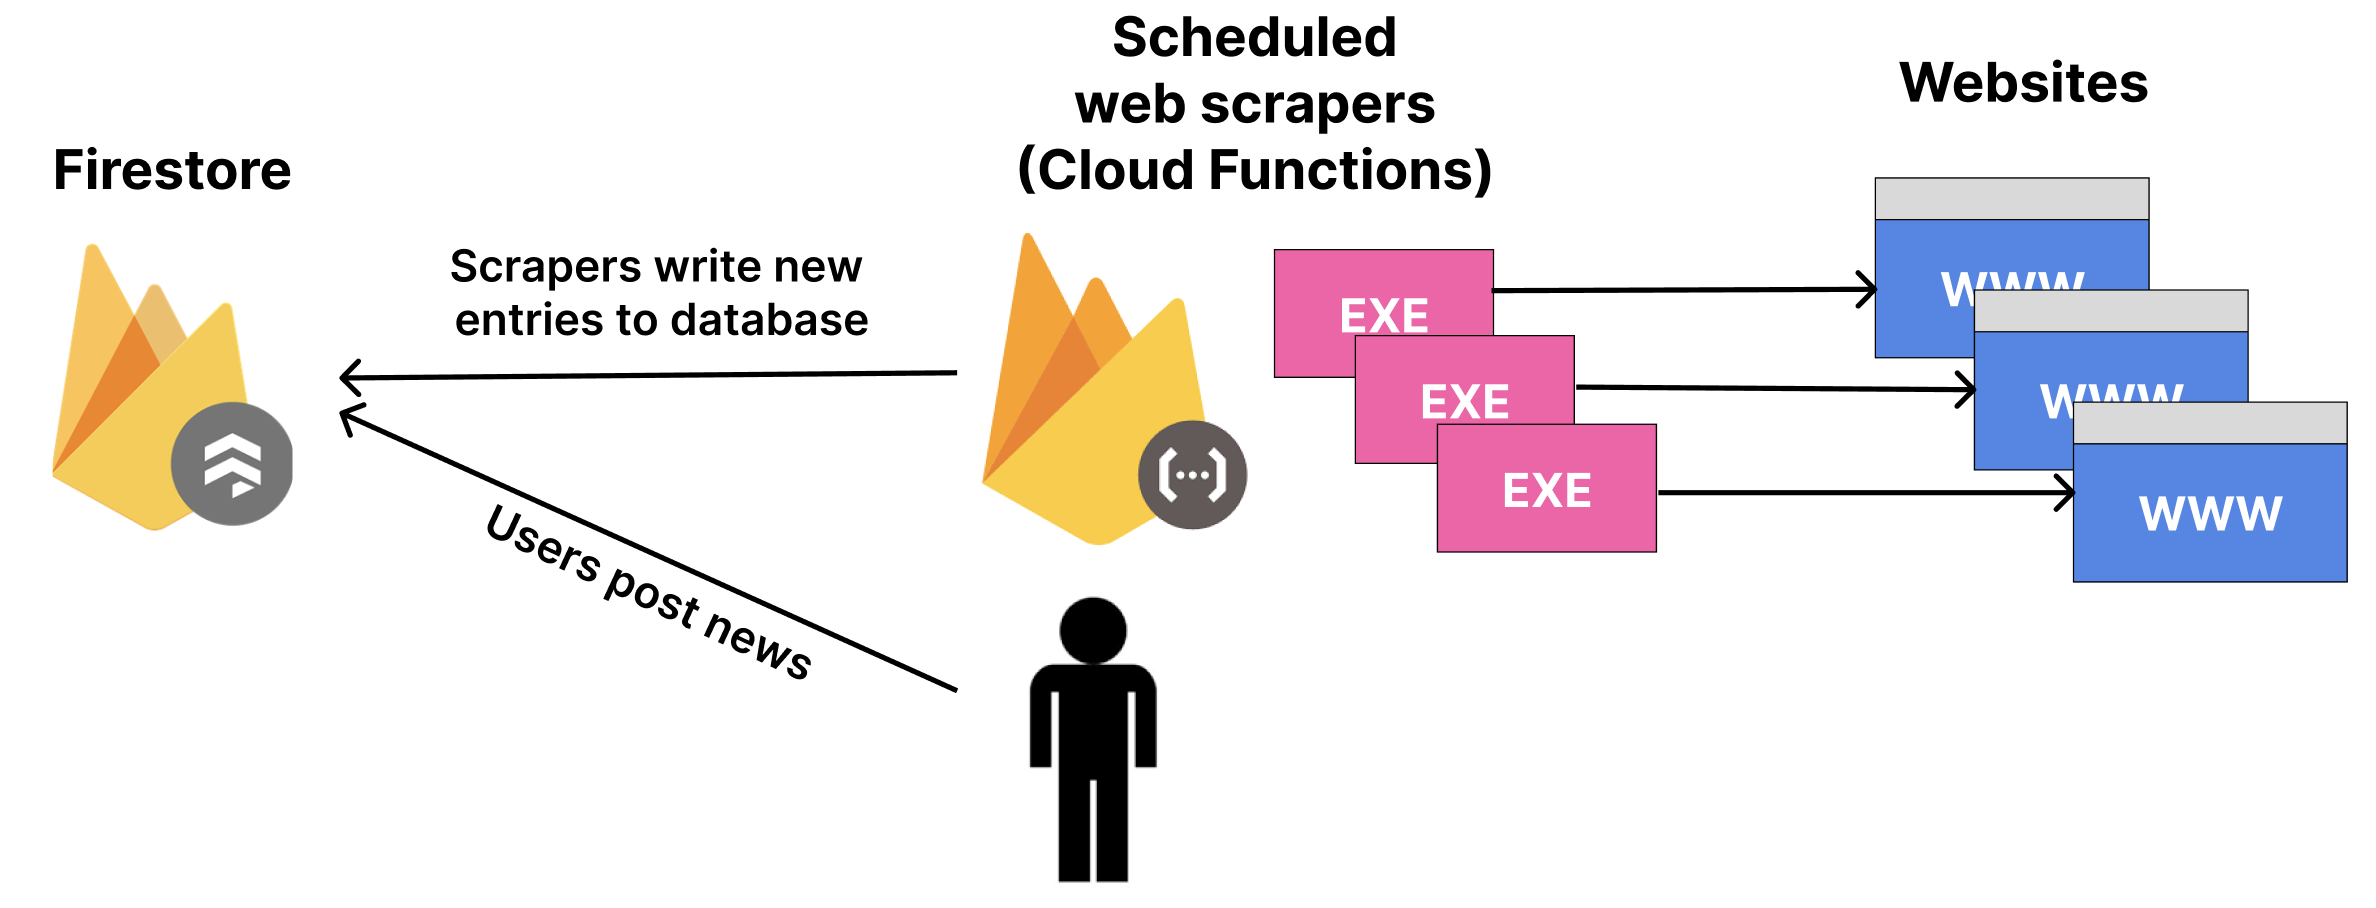
\includegraphics[width=\textwidth]{figures/app/miscellanous/cloud-functions-pipeline-1.png}
    \caption{Cloud functions pipeline - step 1}
    \label{4:fig:cloud_functions_step_1}
\end{figure}

~

\begin{figure}[ht]
    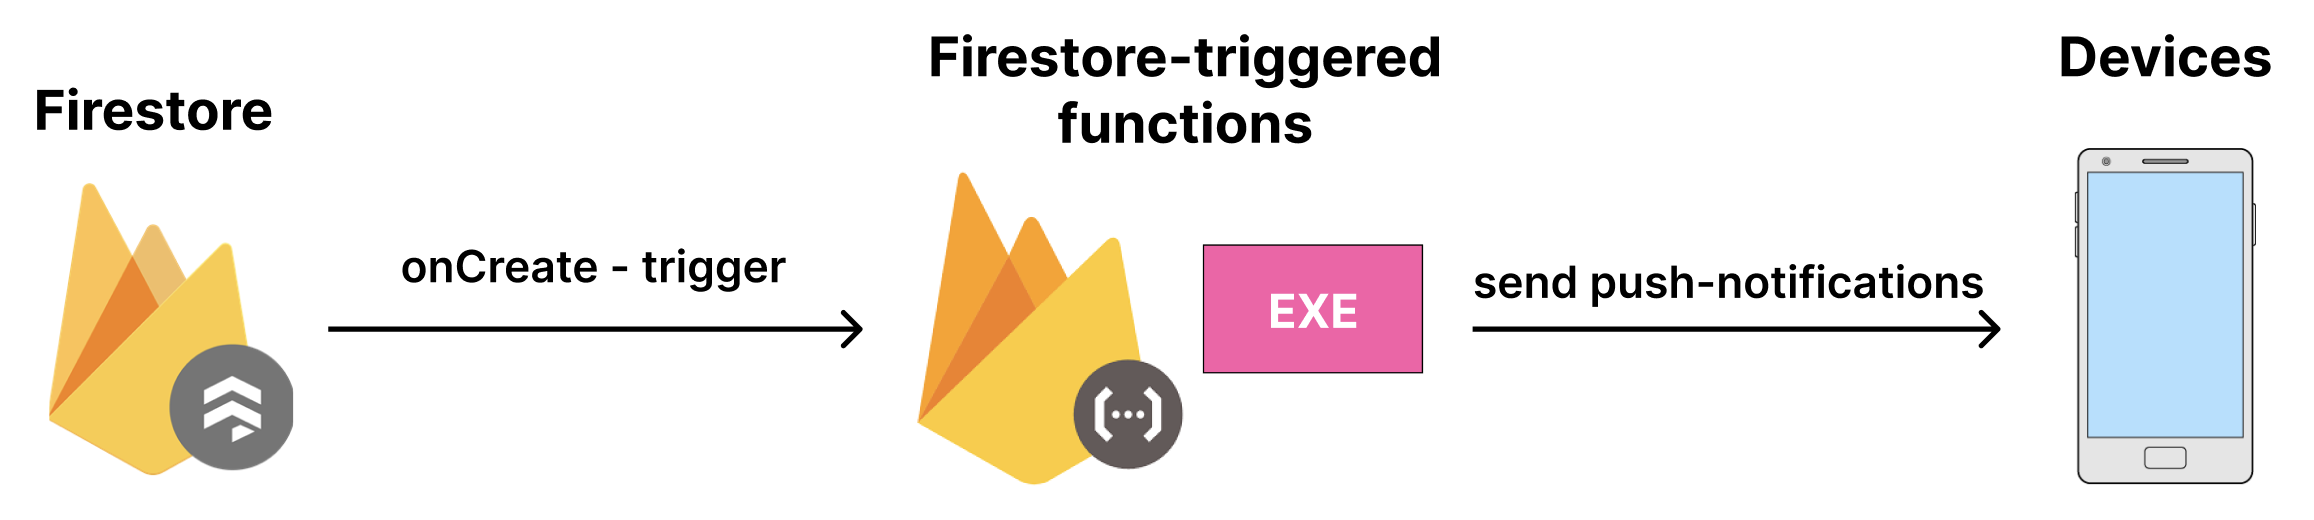
\includegraphics[width=\textwidth]{figures/app/miscellanous/cloud-functions-pipeline-2.png}
    \caption{Cloud functions pipeline - step 2}
    \label{4:fig:cloud_functions_step_2}
\end{figure}

\subsection{Web scrapers} \label{5:web-scrapers}

Our web scrapers search the available content on the RSS feeds of our targeted faculty platforms. RSS or "Really Simple Syndication" is a standard technology that enables third-party applications to subscribe to one platform's feed and was an essential component in the emergence of content aggregators on the Internet. These RSS feeds consist primarily of text files that contain posts, articles or updates, and the standard markup language for these files is XML. As a result, we needed to have our scrapers retrieve and parse this format before inserting new entries into the database.

~
The XML data contains relevant information about a post, such as HTML, author or timestamp. To display the content of a post in our app, we need to parse its HTML from the XML document and then convert the HTML into Markdown syntax. We decided to use Markdown for displaying and publishing posts because it is an increasingly popular markup language that users and programs can easily interpret. According to this Google Developer post\footnote{https://developers.google.com/style/markdown}, Markdown is easier to write by humans, whereas HTML is more expressive in terms of visual elements. Moreover, we have specialized widget components in our Flutter code that can render Markdown on the screen.

~
Finally, when we started to import posts into our app, we noticed that most of them did not lose any information during the scraping process and preserved their original layout. On the other hand, there were posts that had some original styling in place and could not be fully translated into Markdown syntax. As a consequence, these posts lost expressiveness or, worse, valuable information that rendered them useless. However, the vast majority of posts did not face any issues, and therefore, we feel pretty confident with the current result. Additionally, since each web scraper runs in a separate function independently from the others, the current architecture can be easily extended with more scrapers in the future. 


\subsection{Firebase Cloud Messaging and Notifications} \label{5:notifications}

Due to hardware limitations during the development process, our push-notifications system is tested and currently works only on Android devices. According to this documentation\footnote{https://firebase.flutter.dev/docs/messaging/apple-integration/}, to integrate \textit{Firebase Cloud Messaging} (FCM) with \textit{Apple Push Notification service} (APNs), developers must have an active Apple Developer account and a physical iOS device for receiving messages. For the purpose of this section, we will refer only to Android devices.

~
Android apps subscribe to notification channels in the background and handle notifications using defined handlers. Our Android app could be in three main states when listening to notifications: \textbf{foreground} (the app is active on the screen), \textbf{background} (the app is not visible on the screen) and \textbf{terminated} (the app process is shut down). For each of these states, we had to define callback functions that treat the incoming messages.

~
As previously mentioned at \textbf{section \ref{5:models}}, Firebase uses special registration tokens to target messages to devices. Upon creating a new entry in our news collection, the system pushes messages to all available devices, and the logic that decides whether to show a notification resides on the client side.

~
For the purpose of our news aggregator module, we set up the push notifications system from the ground up. Therefore, other features from the \textbf{ACS UPB Mobile} app could benefit from this system in the future since independent notification channels could be easily set up on our implemented code base.

\section{Deep-linking}

Deep links are special URLs that send users directly to the installed app instead of a website. For our purpose, we wanted the users to be able to share external links of news items and have them open directly using our app. Unfortunately, due to hardware limitations, we could not test this functionality on iOS devices.

~
To create a deep link in Android, we must register a specific URL pattern in our system that can be identified and mapped back to our app. Therefore, whenever the user searches a specific URL, the Android system checks whether that link can be opened by an available app and forwards the action accordingly.

~
Currently, our functionality is not yet fully complete. While we can open URLs with a specific scheme (e.g. \url{acs://acs.upb.mobile.dev/news-details?guid=<item-reference>}), our end goal is to define HTTPS-based URLs that can either open the app or send the user straight to Google Play Store to download it. To achieve this functionality, we plan on using the \textit{Firebase Dynamic Links}\footnote{https://firebase.google.com/docs/dynamic-links} service in the future once we start releasing new versions of the \textbf{ACS UPB Mobile} app in the Google Play Store.

~
Similarly to the previous push-notification system described at \textbf{\ref{5:notifications}}, there was no existing deep-linking support in the original app. Deep links can trigger various actions within an app and therefore, we believe that our implementation could be reused in the future to support other features. 